\newpage
\section{Sprint 3}

Siguiendo la planificación inicial, el tercer sprint se centra en la implementación del procesado multimedia en el servidor (generación de miniaturas, compresión de imágenes y vídeos, etiquetado basado en metadatos, etc.) y en el cliente móvil la subida de archivos multimedia al servidor y la visualización de los archivos subidos.

El objetivo es entregar un incremento funcional que permita al usuario subir fotos y vídeos desde el móvil, que el servidor procese estos archivos (compresión, miniaturas) y que puedan visualizarse en una galería online básica. Se priorizan historias que permitan una experiencia de usuario completa de subida y visualización, así como la robustez y eficiencia del proceso.

\subsection{Historias de usuario}
A continuación se presentan las historias de usuario y técnicas seleccionadas para este sprint, siguiendo el mismo formato que en los sprints anteriores. El desglose en tareas se realizará posteriormente.

Las historias seleccionadas son las siguientes:
\begin{itemize}
    % Servidor (prioridad máxima)
    \item HU01: Subida de fotos -- 5 PH
    \item HU04: Subida de vídeos -- 5 PH
    \item HT09: Compresión de imágenes -- 5 PH
    \item HT10: Subida concurrente -- 8 PH
    \item HU09: Galería visual -- 5 PH
    \item HT17: Notificaciones de progreso -- 3 PH
    % Cliente móvil (imprescindible para probar subida y visualización)
    \item HU16: Seleccionar fotos -- 3 PH
    \item HU27: Subir vídeos -- 5 PH
    \item HU18: Ver progreso de subida -- 8 PH
\end{itemize}

La suma total de las historias seleccionadas es de \textbf{47 puntos de historia (PH)}. Esta selección se ha ajustado para priorizar el procesado multimedia en el servidor y solo las funcionalidades imprescindibles del cliente móvil, manteniendo una carga realista y coherente con la capacidad demostrada en los sprints anteriores (34–56 PH). Se han dejado fuera historias menos críticas para el objetivo de este sprint, como la cancelación de subida, sincronización manual, galería online avanzada, manejo de errores de red y estadísticas de copia, que se abordarán en sprints posteriores.

\subsection{Descomposición en tareas de desarrollo}

% HU01: Subida de fotos
\begin{table}[H]
    \begin{center}
        \begin{tabularx}{\textwidth}{|l|X|l|}
            \hline
            \textbf{Identificador HU01} &
            \textbf{Como usuario, quiero subir varias fotos desde mi móvil para tener una copia de seguridad en mi servidor} &
            \textbf{Estimación: 5 PH}\\
            \hline
            \multicolumn{3}{|p{\textwidth}|}{
                \begin{minipage}{\textwidth}
                    \centering
                    \vspace{0.5em}
                    \begin{tabular}{|l|p{8cm}|r|}
                        \hline
                        \textbf{Identificador} & \textbf{Título de la tarea de desarrollo} & \makecell{\textbf{Estimación}\\\textbf{(h)}} \\
                        \hline
                        Tarea 01-1 & Implementar endpoint de subida de fotos (backend) & 2 \\
                        \hline
                        Tarea 01-2 & Validar y almacenar archivos recibidos & 1.5 \\
                        \hline
                        Tarea 01-3 & Integrar con sistema de almacenamiento (local o cloud) & 1 \\
                        \hline
                        Tarea 01-4 & Pruebas unitarias y de integración & 1 \\
                        \hline
                        Tarea 01-5 & Documentar endpoint & 0.5 \\
                        \hline
                    \end{tabular}
                    \vspace{0.5em}
                \end{minipage}
            } \\
            \hline
            \multicolumn{3}{|p{\textwidth}|}{
                \textbf{Pruebas de aceptación:}
                \begin{itemize}
                    \item El usuario puede subir una o varias fotos desde el móvil.
                    \item Los archivos se almacenan correctamente en el servidor.
                    \item El endpoint rechaza archivos no válidos.
                \end{itemize}
            }\\
            \hline
            \multicolumn{3}{|p{\textwidth}|}{
                \textbf{Observaciones:}
                \begin{itemize}
                    \item El endpoint debe ser seguro y validar el tipo de archivo.
                    \item Es necesario implementar un límite de tamaño máximo de archivo.
                \end{itemize}
            }\\
            \hline
        \end{tabularx}
    \end{center}
\end{table}

% HU04: Subida de vídeos
\begin{table}[H]
    \begin{center}
        \begin{tabularx}{\textwidth}{|l|X|l|}
            \hline
            \textbf{Identificador HU04} &
            \textbf{Como usuario, quiero subir vídeos desde mi móvil para tener una copia de seguridad en mi servidor} &
            \textbf{Estimación: 5 PH}\\
            \hline
            \multicolumn{3}{|p{\textwidth}|}{
                \begin{minipage}{\textwidth}
                    \centering
                    \vspace{0.5em}
                    \begin{tabular}{|l|p{8cm}|r|}
                        \hline
                        \textbf{Identificador} & \textbf{Título de la tarea de desarrollo} & \makecell{\textbf{Estimación}\\\textbf{(h)}} \\
                        \hline
                        Tarea 04-1 & Implementar endpoint de subida de vídeos & 2 \\
                        \hline
                        Tarea 04-2 & Validar y almacenar vídeos recibidos & 1.5 \\
                        \hline
                        Tarea 04-3 & Integrar con sistema de almacenamiento & 1 \\
                        \hline
                        Tarea 04-4 & Pruebas unitarias y de integración & 1 \\
                        \hline
                        Tarea 04-5 & Documentar endpoint & 0.5 \\
                        \hline
                    \end{tabular}
                    \vspace{0.5em}
                \end{minipage}
            } \\
            \hline
            \multicolumn{3}{|p{\textwidth}|}{
                \textbf{Pruebas de aceptación:}
                \begin{itemize}
                    \item El usuario puede subir uno o varios vídeos desde el móvil.
                    \item Los archivos se almacenan correctamente en el servidor.
                    \item El endpoint rechaza archivos no válidos.
                \end{itemize}
            }\\
            \hline
            \multicolumn{3}{|p{\textwidth}|}{
                \textbf{Observaciones:}
                \begin{itemize}
                    \item El endpoint debe ser seguro y validar el tipo de archivo.
                    \item Es necesario implementar un límite de tamaño máximo de archivo.
                \end{itemize}
            }\\
            \hline
        \end{tabularx}
    \end{center}
\end{table}

% HT09: Compresión de imágenes
\begin{table}[H]
    \begin{center}
        \begin{tabularx}{\textwidth}{|l|X|l|}
            \hline
            \textbf{Identificador HT09} &
            \textbf{Comprimir imágenes tras la subida para optimizar almacenamiento y ancho de banda} &
            \textbf{Estimación: 5 PH}\\
            \hline
            \multicolumn{3}{|p{\textwidth}|}{
                \begin{minipage}{\textwidth}
                    \centering
                    \vspace{0.5em}
                    \begin{tabular}{|l|p{8cm}|r|}
                        \hline
                        \textbf{Identificador} & \textbf{Título de la tarea de desarrollo} & \makecell{\textbf{Estimación}\\\textbf{(h)}} \\
                        \hline
                        Tarea 09-1T & Investigar y seleccionar librería de compresión & 1 \\
                        \hline
                        Tarea 09-2T & Implementar lógica de compresión tras subida & 2 \\
                        \hline
                        Tarea 09-3T & Pruebas de compresión y calidad & 1 \\
                        \hline
                        Tarea 09-4T & Manejo de errores y logs & 0.5 \\
                        \hline
                        Tarea 09-5T & Documentar proceso & 0.5 \\
                        \hline
                    \end{tabular}
                    \vspace{0.5em}
                \end{minipage}
            } \\
            \hline
            \multicolumn{3}{|p{\textwidth}|}{
                \textbf{Pruebas de aceptación:}
                \begin{itemize}
                    \item Las imágenes subidas se comprimen automáticamente.
                    \item La calidad de las imágenes comprimidas es aceptable.
                    \item El proceso de compresión no bloquea la subida.
                \end{itemize}
            }\\
            \hline
            \multicolumn{3}{|p{\textwidth}|}{
                \textbf{Observaciones:}
                \begin{itemize}
                    \item Seleccionar un balance adecuado entre compresión y calidad.
                \end{itemize}
            }\\
            \hline
        \end{tabularx}
    \end{center}
\end{table}

% HT10: Subida concurrente
\begin{table}[H]
    \begin{center}
        \begin{tabularx}{\textwidth}{|l|X|l|}
            \hline
            \textbf{Identificador HT10} &
            \textbf{Permitir la subida concurrente de archivos para mejorar la eficiencia} &
            \textbf{Estimación: 8 PH}\\
            \hline
            \multicolumn{3}{|p{\textwidth}|}{
                \begin{minipage}{\textwidth}
                    \centering
                    \vspace{0.5em}
                    \begin{tabular}{|l|p{8cm}|r|}
                        \hline
                        \textbf{Identificador} & \textbf{Título de la tarea de desarrollo} & \makecell{\textbf{Estimación}\\\textbf{(h)}} \\
                        \hline
                        Tarea 10-1 & Diseñar arquitectura para subida concurrente & 1.5 \\
                        \hline
                        Tarea 10-2 & Implementar manejo de múltiples subidas simultáneas & 2 \\
                        \hline
                        Tarea 10-3 & Control de concurrencia y límites & 1.5 \\
                        \hline
                        Tarea 10-4 & Pruebas de estrés y concurrencia & 1.5 \\
                        \hline
                        Tarea 10-5 & Logs y métricas & 0.5 \\
                        \hline
                        Tarea 10-6 & Documentar solución & 0.5 \\
                        \hline
                    \end{tabular}
                    \vspace{0.5em}
                \end{minipage}
            } \\
            \hline
            \multicolumn{3}{|p{\textwidth}|}{
                \textbf{Pruebas de aceptación:}
                \begin{itemize}
                    \item El servidor acepta varias subidas simultáneas sin errores.
                    \item Se limita el número de subidas concurrentes según configuración.
                    \item El rendimiento mejora respecto a la subida secuencial.
                \end{itemize}
            }\\
            \hline
            \multicolumn{3}{|p{\textwidth}|}{
                \textbf{Observaciones:}
                \begin{itemize}
                    \item Es importante evitar bloqueos y condiciones de carrera.
                \end{itemize}
            }\\
            \hline
        \end{tabularx}
    \end{center}
\end{table}

% HU09: Galería visual
\begin{table}[H]
    \begin{center}
        \begin{tabularx}{\textwidth}{|l|X|l|}
            \hline
            \textbf{Identificador HU09} &
            \textbf{Como usuario, quiero ver una galería online de mis archivos subidos} &
            \textbf{Estimación: 5 PH}\\
            \hline
            \multicolumn{3}{|p{\textwidth}|}{
                \begin{minipage}{\textwidth}
                    \centering
                    \vspace{0.5em}
                    \begin{tabular}{|l|p{8cm}|r|}
                        \hline
                        \textbf{Identificador} & \textbf{Título de la tarea de desarrollo} & \makecell{\textbf{Estimación}\\\textbf{(h)}} \\
                        \hline
                        Tarea 09-1U & Implementar endpoint para listar archivos multimedia & 1.5 \\
                        \hline
                        Tarea 09-2U & Generar miniaturas para galería & 1.5 \\
                        \hline
                        Tarea 09-3U & Implementar paginación/búsqueda básica & 1 \\
                        \hline
                        Tarea 09-4U & Pruebas de visualización & 0.5 \\
                        \hline
                        Tarea 09-5U & Documentar endpoint & 0.5 \\
                        \hline
                    \end{tabular}
                    \vspace{0.5em}
                \end{minipage}
            } \\
            \hline
            \multicolumn{3}{|p{\textwidth}|}{
                \textbf{Pruebas de aceptación:}
                \begin{itemize}
                    \item El usuario puede ver una galería online de sus archivos subidos.
                    \item Las miniaturas se generan correctamente.
                    \item La galería soporta paginación o búsqueda básica.
                \end{itemize}
            }\\
            \hline
            \multicolumn{3}{|p{\textwidth}|}{
                \textbf{Observaciones:}
                \begin{itemize}
                    \item La galería debe ser eficiente y escalable.
                \end{itemize}
            }\\
            \hline
        \end{tabularx}
    \end{center}
\end{table}

% HT17: Notificaciones de progreso
\begin{table}[H]
    \begin{center}
        \begin{tabularx}{\textwidth}{|l|X|l|}
            \hline
            \textbf{Identificador HT17} &
            \textbf{Notificar al cliente el progreso de la subida de archivos} &
            \textbf{Estimación: 3 PH}\\
            \hline
            \multicolumn{3}{|p{\textwidth}|}{
                \begin{minipage}{\textwidth}
                    \centering
                    \vspace{0.5em}
                    \begin{tabular}{|l|p{8cm}|r|}
                        \hline
                        \textbf{Identificador} & \textbf{Título de la tarea de desarrollo} & \makecell{\textbf{Estimación}\\\textbf{(h)}} \\
                        \hline
                        Tarea 17-1 & Implementar sistema de notificaciones de progreso (API) & 1 \\
                        \hline
                        Tarea 17-2 & Integrar con endpoints de subida & 0.5 \\
                        \hline
                        Tarea 17-3 & Pruebas y logs & 0.5 \\
                        \hline
                        Tarea 17-4 & Documentar & 0.5 \\
                        \hline
                    \end{tabular}
                    \vspace{0.5em}
                \end{minipage}
            } \\
            \hline
            \multicolumn{3}{|p{\textwidth}|}{
                \textbf{Pruebas de aceptación:}
                \begin{itemize}
                    \item El cliente recibe notificaciones de progreso durante la subida.
                    \item El sistema informa correctamente de errores o finalización.
                \end{itemize}
            }\\
            \hline
            \multicolumn{3}{|p{\textwidth}|}{
                \textbf{Observaciones:}
                \begin{itemize}
                    \item Puede usarse WebSocket, SSE o polling según la arquitectura.
                \end{itemize}
            }\\
            \hline
        \end{tabularx}
    \end{center}
\end{table}

% HU16: Seleccionar fotos (móvil)
\begin{table}[H]
    \begin{center}
        \begin{tabularx}{\textwidth}{|l|X|l|}
            \hline
            \textbf{Identificador HU16} &
            \textbf{Como usuario, quiero seleccionar fotos desde la galería del móvil para subirlas al servidor} &
            \textbf{Estimación: 3 PH}\\
            \hline
            \multicolumn{3}{|p{\textwidth}|}{
                \begin{minipage}{\textwidth}
                    \centering
                    \vspace{0.5em}
                    \begin{tabular}{|l|p{8cm}|r|}
                        \hline
                        \textbf{Identificador} & \textbf{Título de la tarea de desarrollo} & \makecell{\textbf{Estimación}\\\textbf{(h)}} \\
                        \hline
                        Tarea 16-1 & Implementar selector de fotos en el cliente móvil & 1.5 \\
                        \hline
                        Tarea 16-2 & Integrar con permisos del sistema & 1 \\
                        \hline
                        Tarea 16-3 & Pruebas en dispositivos reales & 0.5 \\
                        \hline
                    \end{tabular}
                    \vspace{0.5em}
                \end{minipage}
            } \\
            \hline
            \multicolumn{3}{|p{\textwidth}|}{
                \textbf{Pruebas de aceptación:}
                \begin{itemize}
                    \item El usuario puede seleccionar una o varias fotos desde la galería.
                    \item Se solicitan los permisos necesarios solo cuando es necesario.
                \end{itemize}
            }\\
            \hline
            \multicolumn{3}{|p{\textwidth}|}{
                \textbf{Observaciones:}
            }\\
            \hline
        \end{tabularx}
    \end{center}
\end{table}

% HU27: Subir vídeos (móvil)
\begin{table}[H]
    \begin{center}
        \begin{tabularx}{\textwidth}{|l|X|l|}
            \hline
            \textbf{Identificador HU27} &
            \textbf{Como usuario, quiero seleccionar y subir vídeos desde el móvil al servidor} &
            \textbf{Estimación: 5 PH}\\
            \hline
            \multicolumn{3}{|p{\textwidth}|}{
                \begin{minipage}{\textwidth}
                    \centering
                    \vspace{0.5em}
                    \begin{tabular}{|l|p{8cm}|r|}
                        \hline
                        \textbf{Identificador} & \textbf{Título de la tarea de desarrollo} & \makecell{\textbf{Estimación}\\\textbf{(h)}} \\
                        \hline
                        Tarea 27-1 & Implementar selector de vídeos en el cliente móvil & 1 \\
                        \hline
                        Tarea 27-2 & Lógica de subida de vídeos (cliente) & 1.5 \\
                        \hline
                        Tarea 27-3 & Manejo de errores y reintentos & 1 \\
                        \hline
                        Tarea 27-4 & Pruebas en dispositivos reales & 0.5 \\
                        \hline
                        Tarea 27-5 & Documentar flujo & 0.5 \\
                        \hline
                    \end{tabular}
                    \vspace{0.5em}
                \end{minipage}
            } \\
            \hline
            \multicolumn{3}{|p{\textwidth}|}{
                \textbf{Pruebas de aceptación:}
                \begin{itemize}
                    \item El usuario puede seleccionar y subir uno o varios vídeos.
                    \item El sistema maneja correctamente errores de red y reintentos.
                \end{itemize}
            }\\
            \hline
            \multicolumn{3}{|p{\textwidth}|}{
                \textbf{Observaciones:}
                \begin{itemize}
                    \item Probar con vídeos de diferentes tamaños y formatos.
                \end{itemize}
            }\\
            \hline
        \end{tabularx}
    \end{center}
\end{table}

% HU18: Ver progreso de subida (móvil)
\begin{table}[H]
    \begin{center}
        \begin{tabularx}{\textwidth}{|l|X|l|}
            \hline
            \textbf{Identificador HU18} &
            \textbf{Como usuario, quiero ver el progreso de la subida de archivos en la app móvil} &
            \textbf{Estimación: 8 PH}\\
            \hline
            \multicolumn{3}{|p{\textwidth}|}{
                \begin{minipage}{\textwidth}
                    \centering
                    \vspace{0.5em}
                    \begin{tabular}{|l|p{8cm}|r|}
                        \hline
                        \textbf{Identificador} & \textbf{Título de la tarea de desarrollo} & \makecell{\textbf{Estimación}\\\textbf{(h)}} \\
                        \hline
                        Tarea 18-1 & Implementar barra/indicador de progreso en UI & 1.5 \\
                        \hline
                        Tarea 18-2 & Integrar con notificaciones de backend & 1.5 \\
                        \hline
                        Tarea 18-3 & Actualización en tiempo real del progreso & 1.5 \\
                        \hline
                        Tarea 18-4 & Pruebas de UX & 1 \\
                        \hline
                        Tarea 18-5 & Manejo de errores y estados & 1 \\
                        \hline
                        Tarea 18-6 & Documentar & 0.5 \\
                        \hline
                    \end{tabular}
                    \vspace{0.5em}
                \end{minipage}
            } \\
            \hline
            \multicolumn{3}{|p{\textwidth}|}{
                \textbf{Pruebas de aceptación:}
                \begin{itemize}
                    \item El usuario ve el progreso de cada archivo subido en tiempo real.
                    \item El sistema informa correctamente de errores o subidas completadas.
                \end{itemize}
            }\\
            \hline
            \multicolumn{3}{|p{\textwidth}|}{
                \textbf{Observaciones:}
                \begin{itemize}
                    \item Probar en diferentes dispositivos y condiciones de red.
                \end{itemize}
            }\\
            \hline
        \end{tabularx}
    \end{center}
\end{table}

\subsection{Diagrama de Gantt}
Una vez definidas las tareas para cada historia de usuario, se ha elaborado un diagrama de Gantt para visualizar la planificación del sprint. Este diagrama muestra el orden de las tareas y su duración estimada:

\begin{figure}[H]
    \begin{center}
        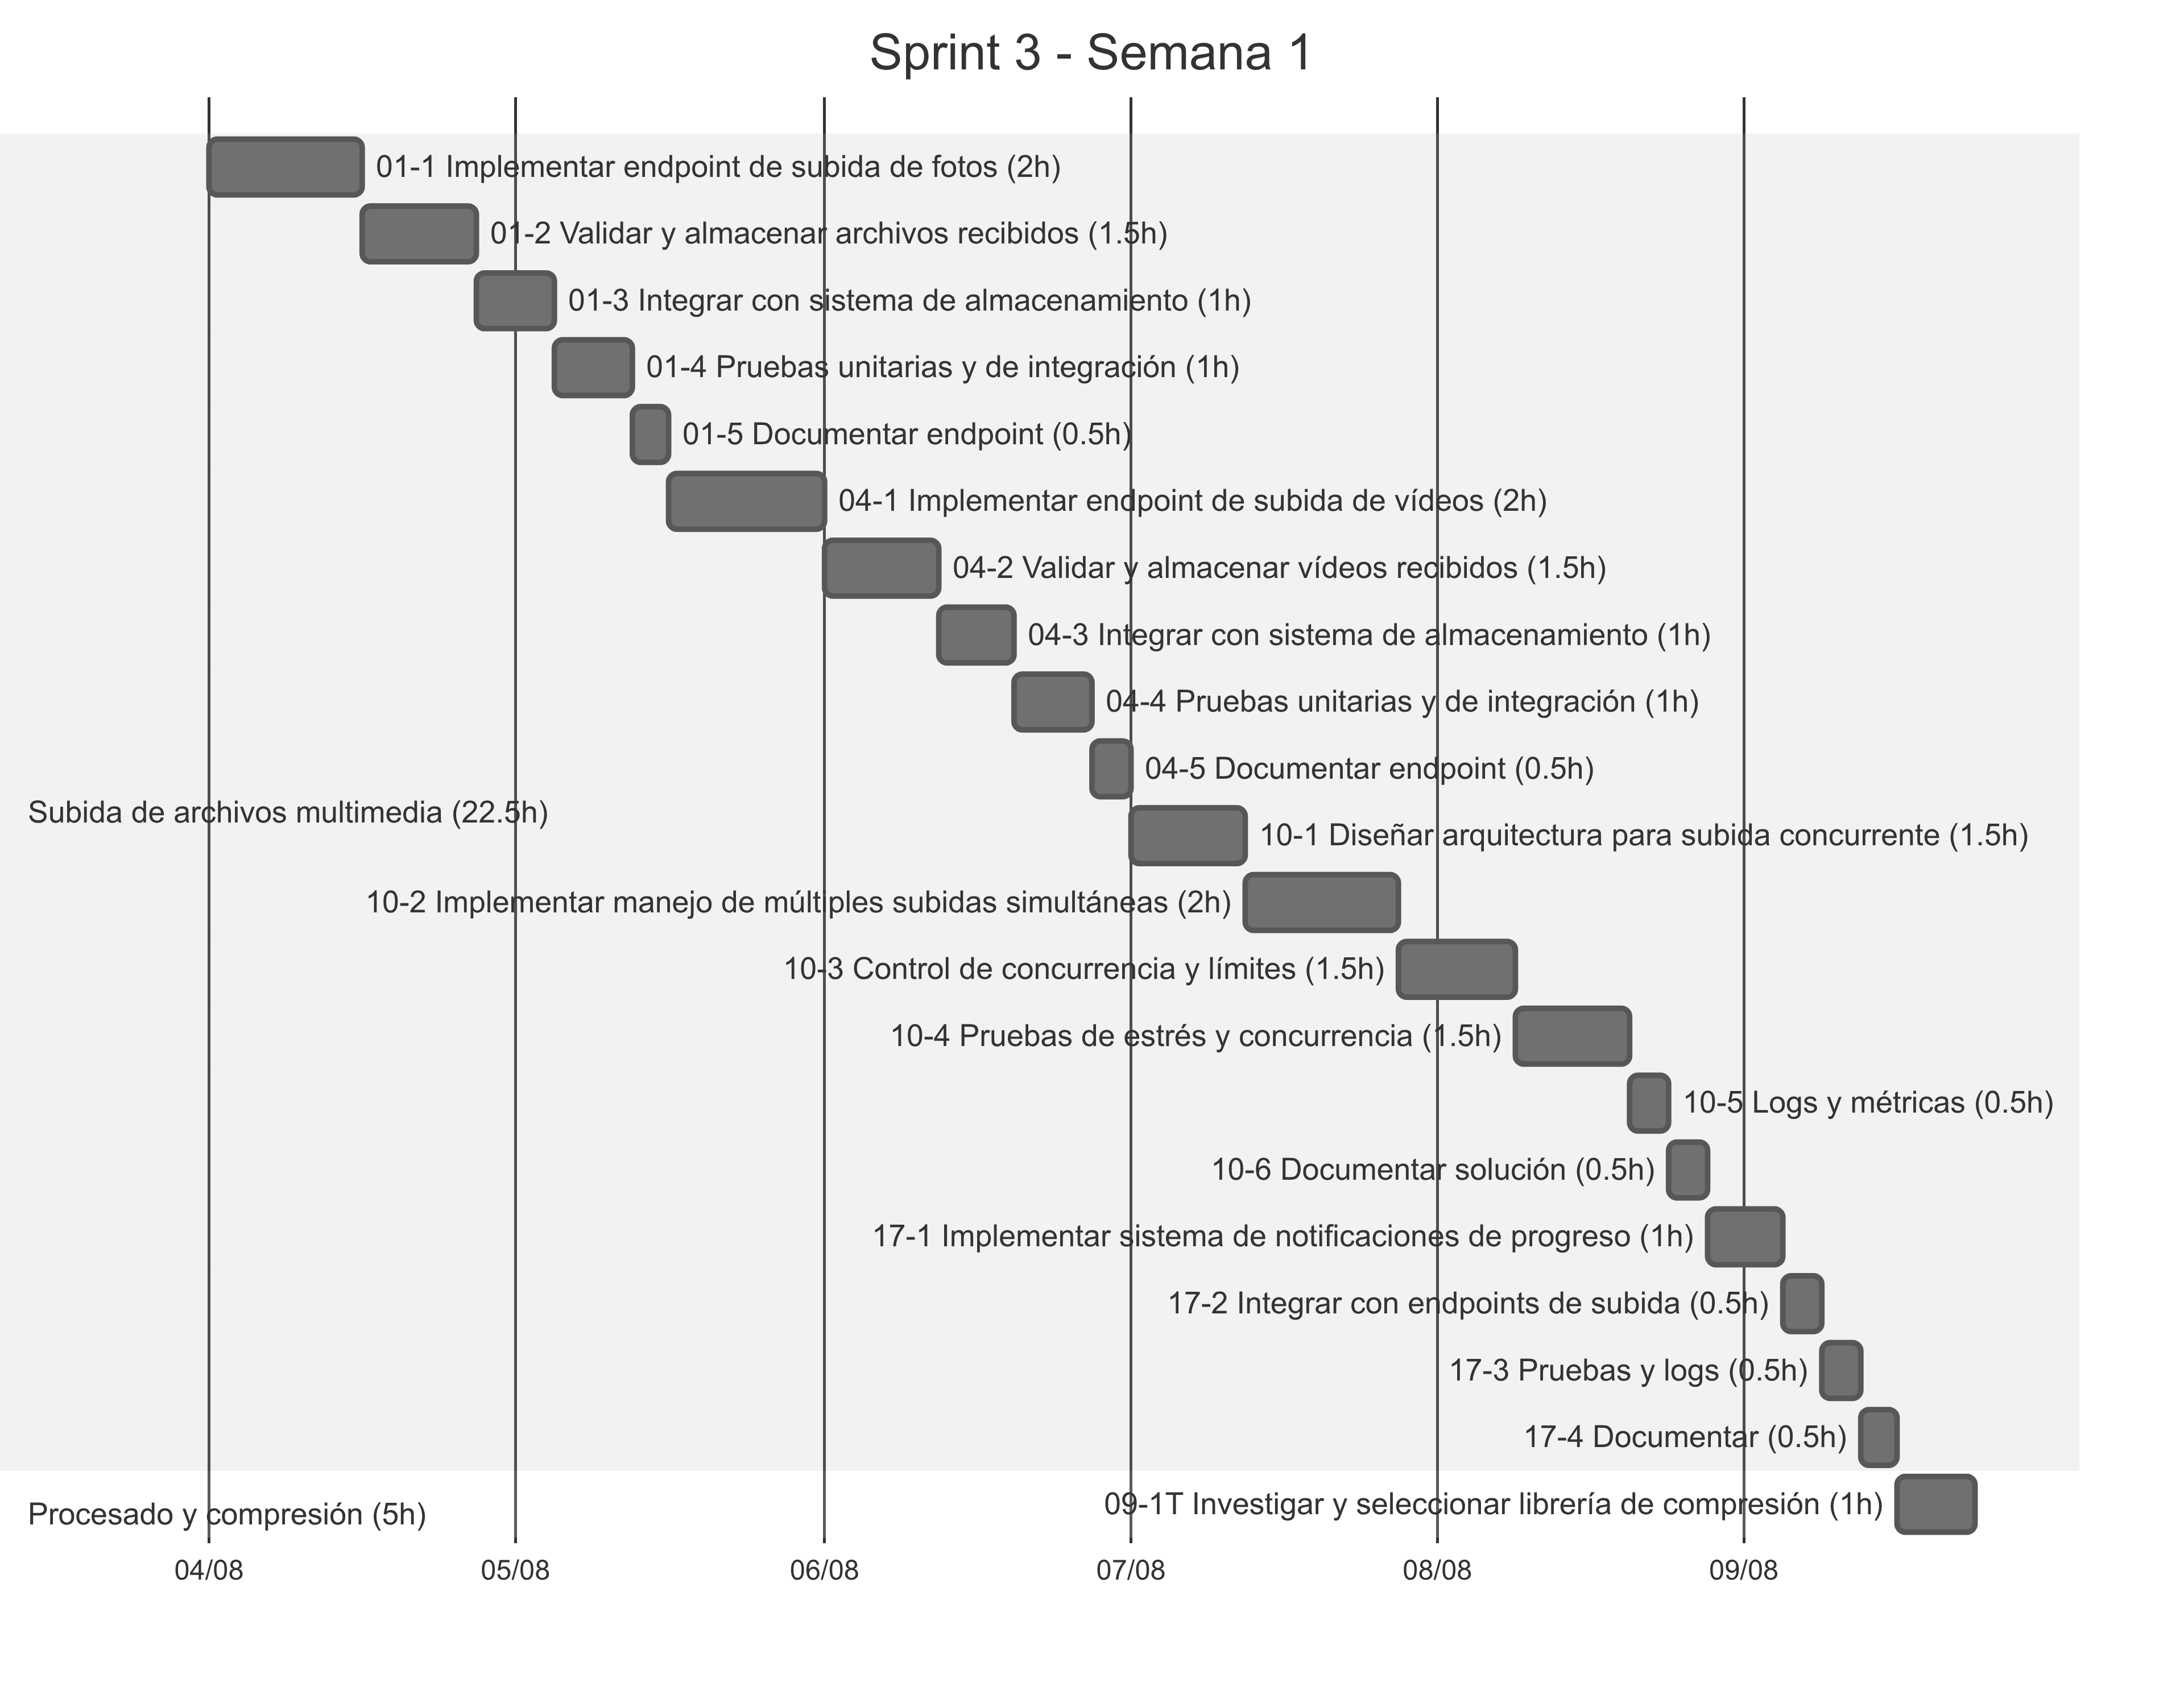
\includegraphics[width=0.8\textwidth]{assets/sprint3/week1-gantt.png}
    \end{center}
    \caption{Diagrama de Gantt de las tareas de la primera semana del sprint 3}\label{fig:gantt-sprint3-week1}
\end{figure}


\begin{figure}[H]
    \begin{center}
        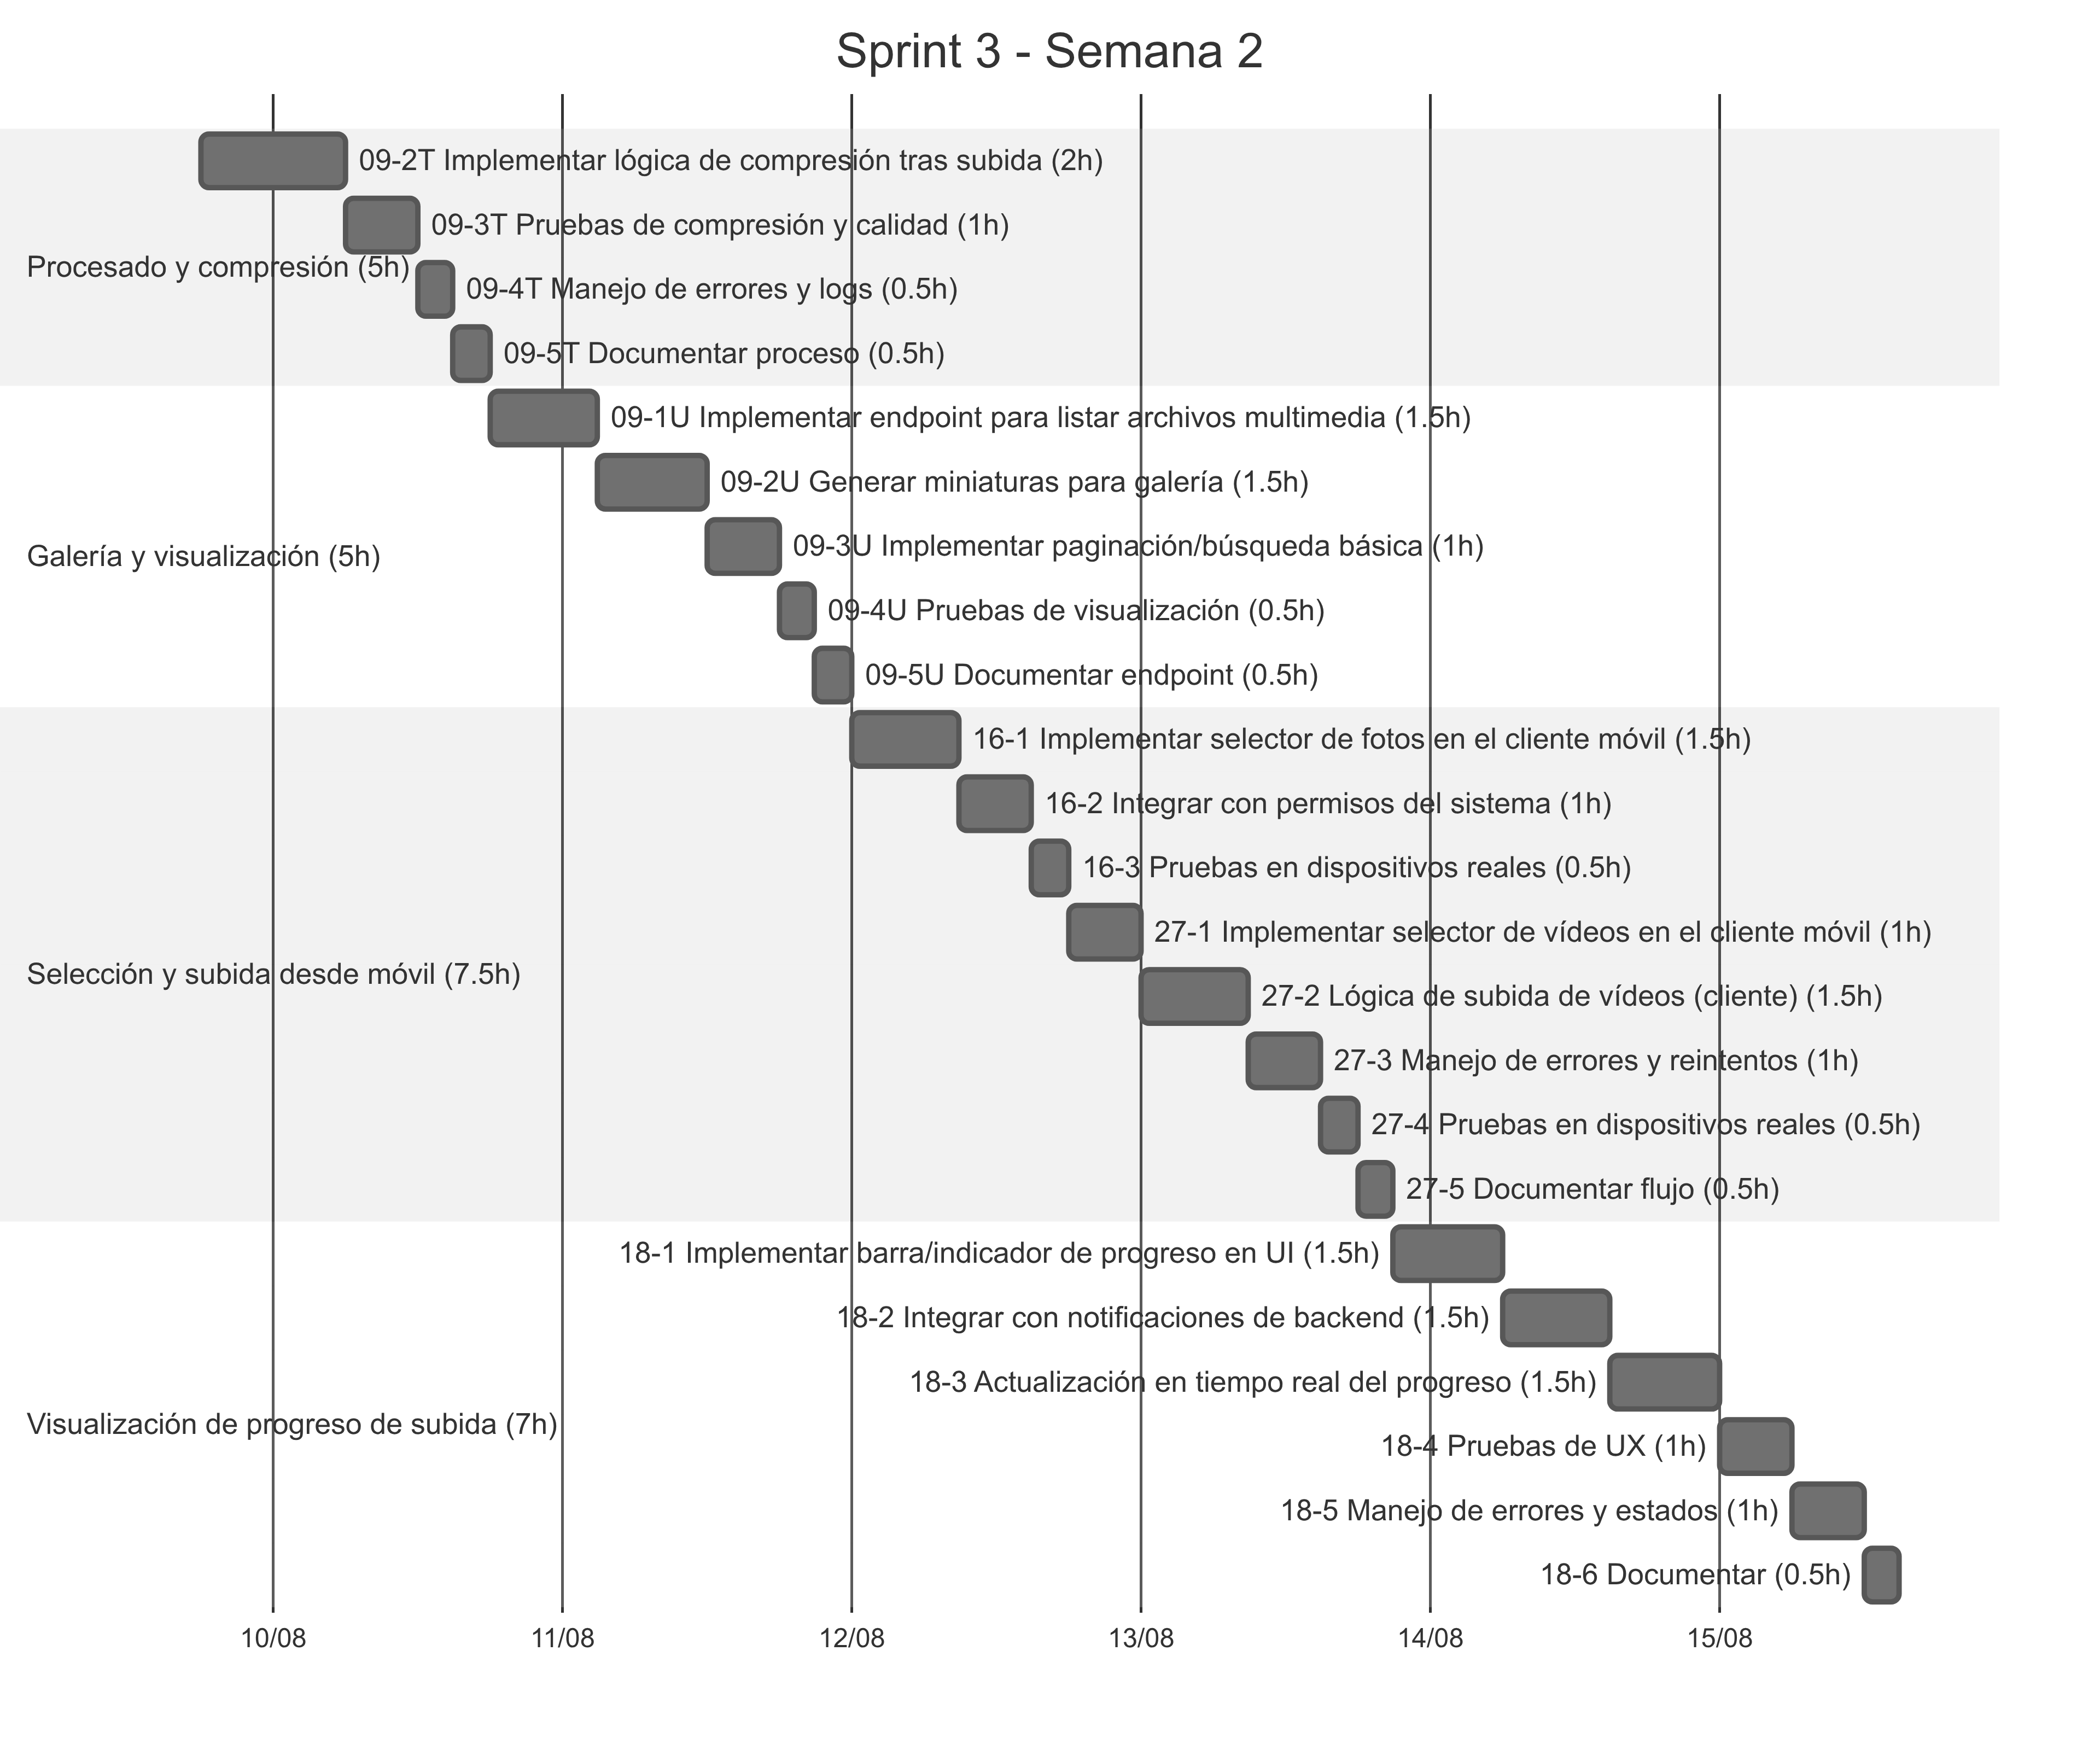
\includegraphics[width=0.8\textwidth]{assets/sprint3/week2-gantt.png}
    \end{center}
    \caption{Diagrama de Gantt de las tareas de la segunda semana del sprint 3}\label{fig:gantt-sprint3-week2}
\end{figure}

En este sprint se han priorizado las tareas relacionadas principalmente con el procesado multimedia en el servidor, dado que en el anterior sprint el enfoque estuvo en el desarrollo de la aplicación móvil.

Las tareas relacionadas con la aplicación móvil de este sprint se centran principalmente en integrar los cambios implementados en el servidor.
Se realiza de esta manera para que al finalizar el sprint 3 tengamos un producto con más valor, puesto que el usuario tendrá la posibilidad de subir fotos y vídeos desde su móvil, que serán procesados en el servidor y podrán visualizarse en una galería online.

\subsection{Diseño detallado e implementación}
La implementación de la subida de archivos multimedia se ha realizado en dos pasos, primero se ha implementado una subida de archivos sencilla, la cual permite subir archivos multimedia al servidor habiendo iniciado sesión, guardando los archivos en MinIO y guardando los metadatos en la base de datos asociados al usuario autenticado.

El flujo que se ha seguido en la implementación ha sido el siguiente:
\begin{figure}[H]
    \begin{center}
        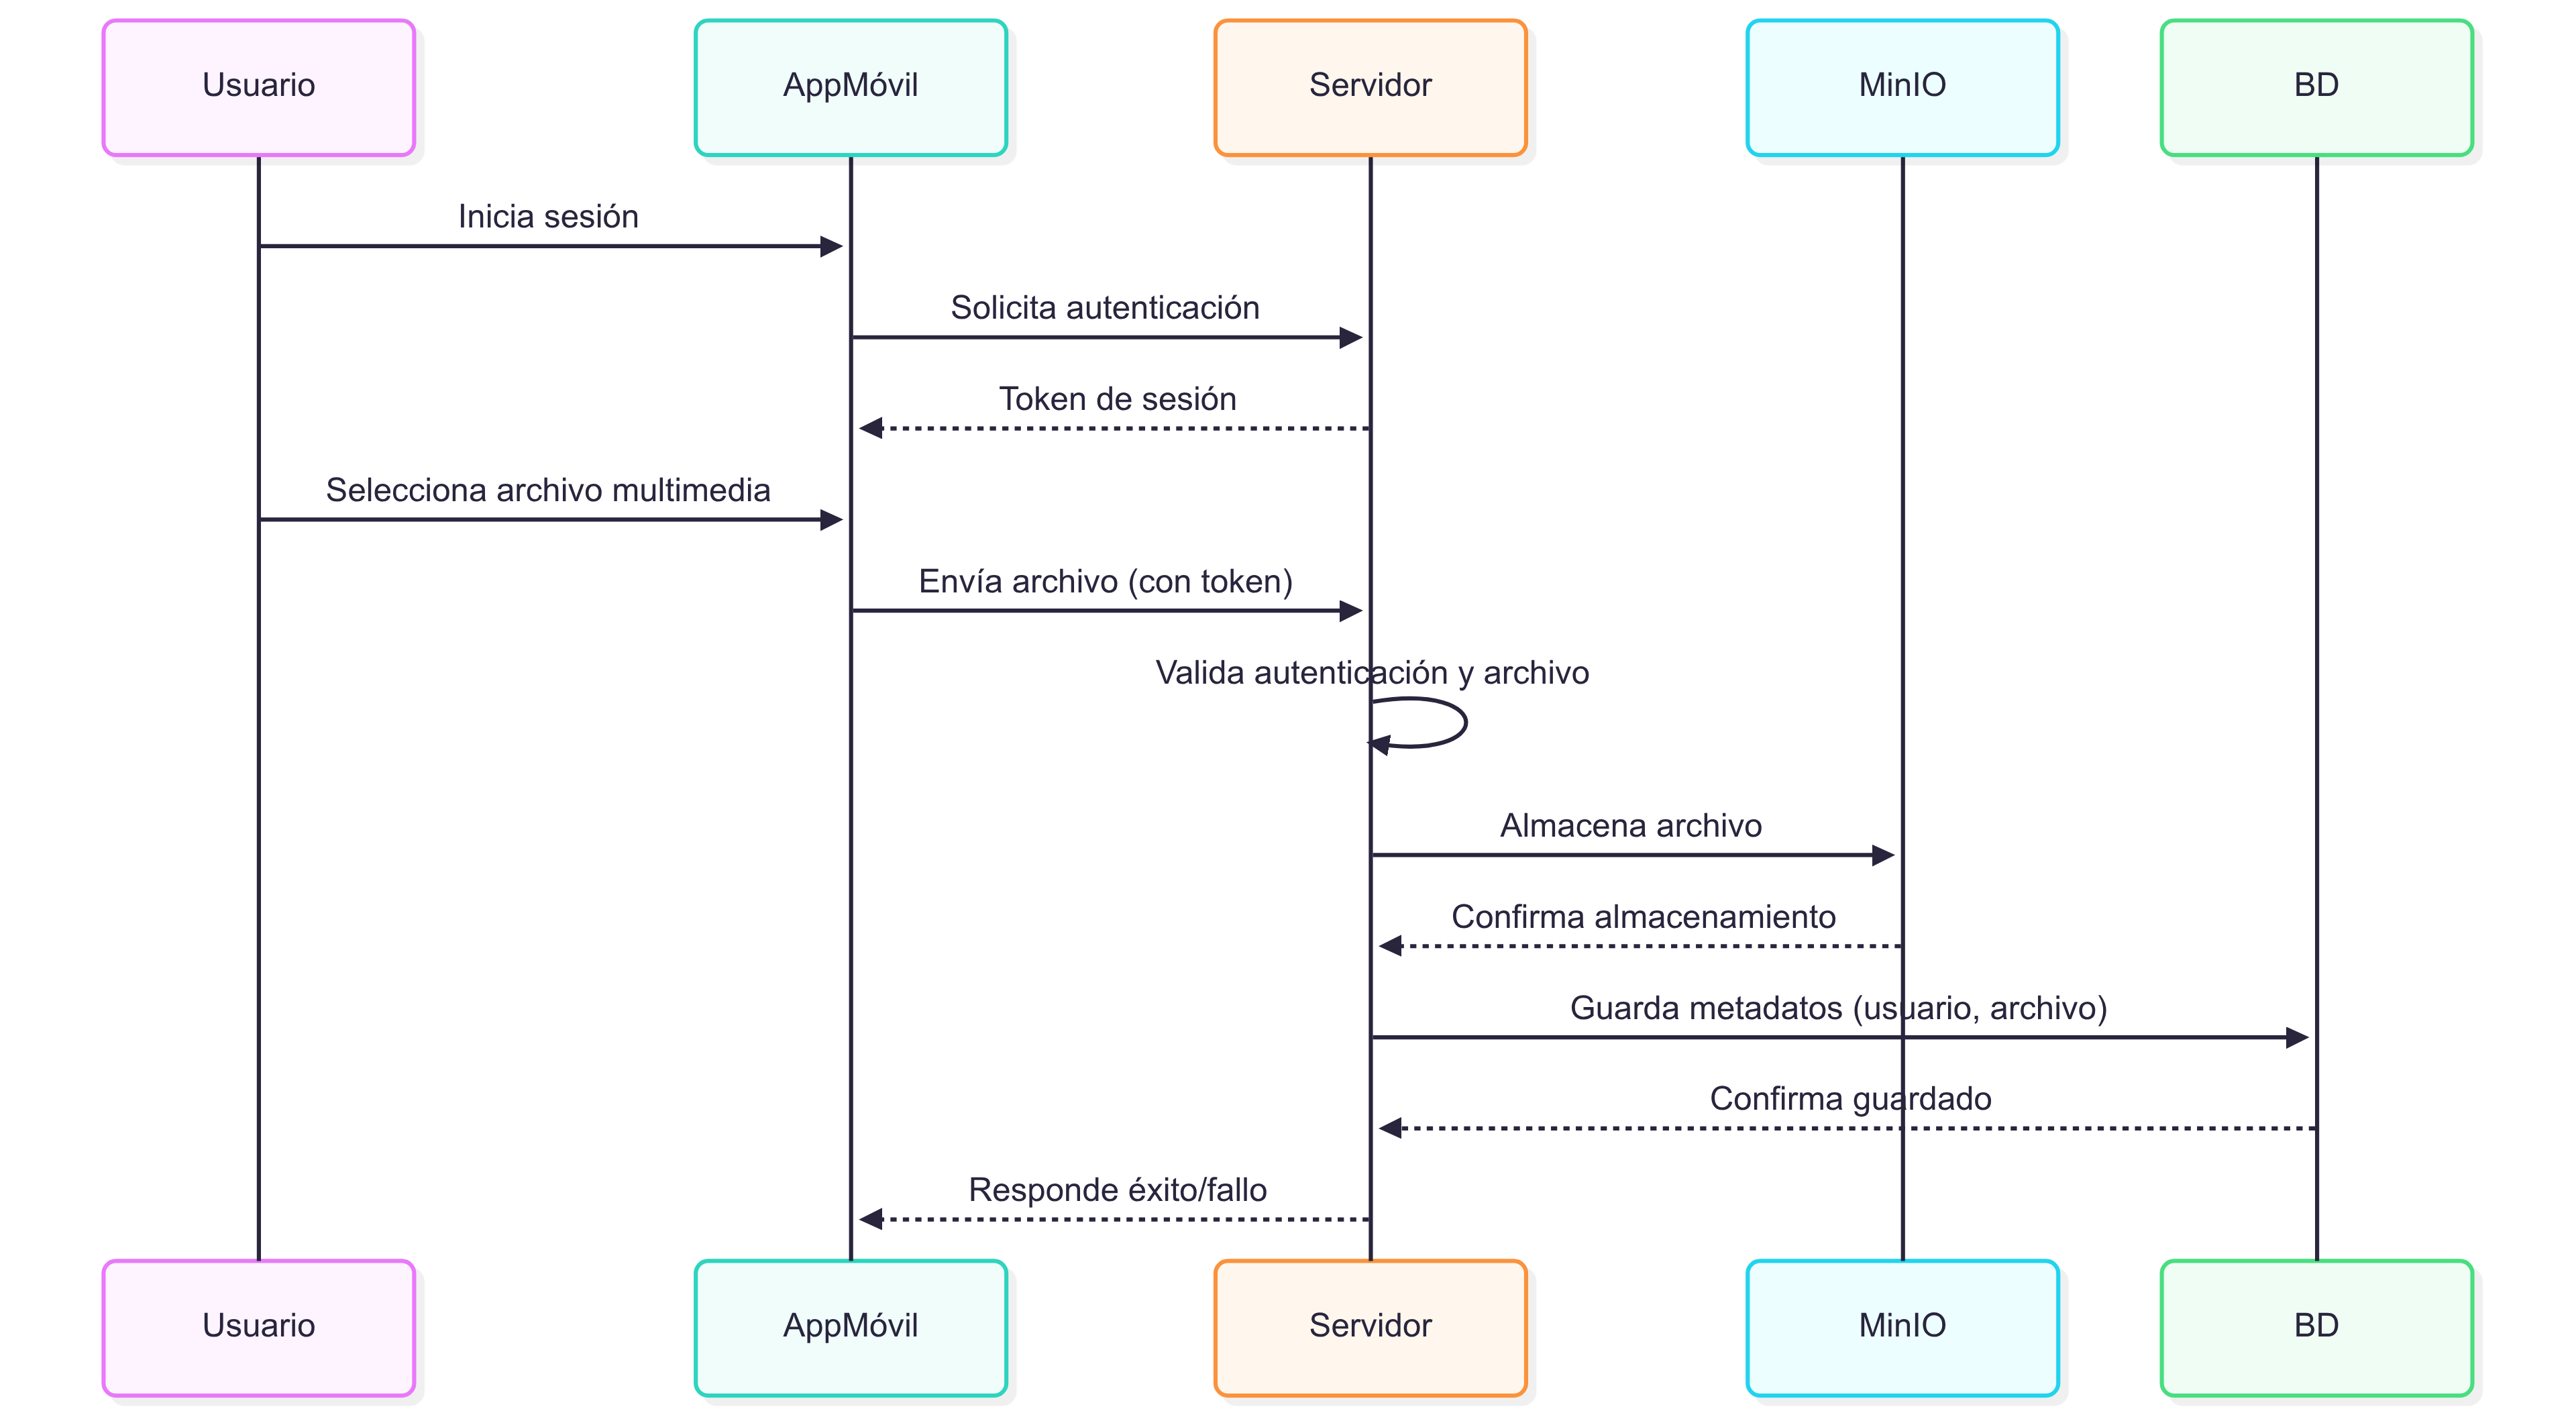
\includegraphics[width=0.95\textwidth]{assets/sprint3/diagrama-subida-archivos.png}
    \end{center}
    \caption{Diagrama de flujo de subida de archivos multimedia}\label{fig:diagrama-flujo-subida-archivos}
\end{figure}

